\chapter{\MakeUppercase{Разработка улучшенного алгоритма обнаружения взаимоблокировок}}

В ходе исследования был разработан алгоритма, который базируется на построение графа, пример которого приведен на Рис. \ref{fig:my_alg-2m2t} для двух потоков.


\begin{figure}[h]
    \centering
    \begin{subfigure}[h]{0.4\textwidth}
        \centering
        \lstinputlisting[language=C]{inc/chapter-first/2m2t-dd.c}
    \end{subfigure}
    \hfill
    \begin{subfigure}[h]{0.4\textwidth}
        \centering
        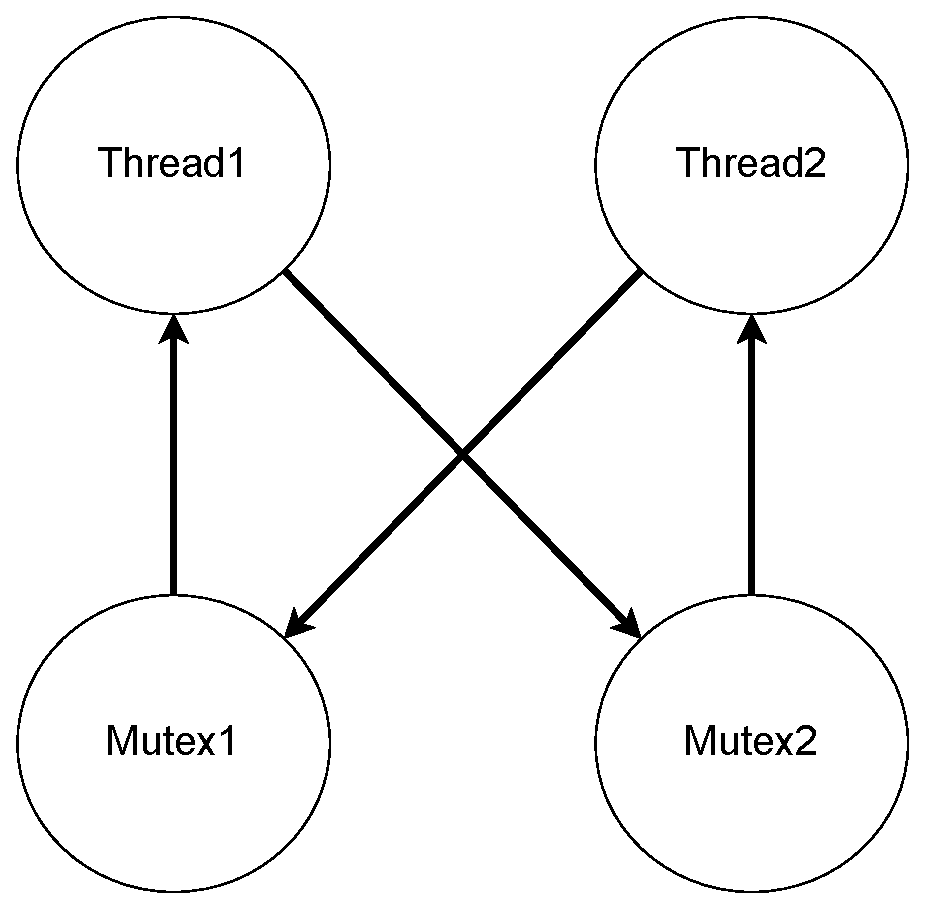
\includegraphics[width=\textwidth]{inc/chapter-second/my_alg-2m2t.eps}
    \end{subfigure}
    \caption{Фрагмент программы с графом обнаружения взаимоблокировок}
    \label{fig:my_alg-2m2t}
\end{figure}

Разработанный алгоритм учитывает, в каком потоке захвачен мьютекс, а также какие еще потоки пытаются захватить этот же мьютекс. История захвата мьютекса представлена на Рис \ref{fig:mutex-algo}.

\begin{figure}[h]
T1: mu1, mu2

T2: mu2, mu1
\caption{История захвата мьютекса в потоках}
\label{fig:mutex-algo}
\end{figure}

На Рис. \ref{fig:mutex-algo} перед двоеточием указано имя потока, а после двоеточия - история захвата мьютексов потоком. Вершинами графа являются потоки и мьютексы. Захваченный потоком мьютекс отображается на графе как направленное ребро от вершины мьютекса к вершине потока. Попытка захвата мьютекса потоком отображается как ребро из вершины потока к вершине мьютекса. Обнаружение цикла в данном графе (как в нашем случае) и будет считаться ситуацией взаимной блокировки, о чем необходимо сообщить пользователю. Из остающихся недостатков данного алгоритма можно отметить, что данный подход применим пока лишь только для обычного mutex.

\subsection{Алгоритм построения графа}

В ходе работы программы необходимо отслеживать действия:
\begin{itemize}
  \item Попытку захвата мьютекса
  \item Захват мьютекса
  \item Освобождение мьютекса
\end{itemize}

Для этих событий необходимо знать поток, который осуществляет это действие, и мьютекс, над которым происходит действие

Алгоритму необходимо хранить список захваченных мьютексов для каждого потока captured[T,mutlist], где T - поток, а mutlist - список захваченных мьютекс в потоке T, а так же хранить для каждого потока попытку захвата мьютекса try[T, M], где T - поток, а M - захваченный мьютекс.

Далее представлен алгоритм для обработки каждого из действий:

\subsubsection{Попытка захвата мьютекса}
\begin{algorithmic}
\Function{TryMutexLock}{thread, mutex}
    \State $try[thread] = mutex$
\EndFunction
\end{algorithmic}

\subsubsection{Захват мьютекса}
\begin{algorithmic}
\Function{MutexLock}{thread, mutex}
    \State $try[thread] = null$
    \If {$thread \notin captured$}
        \State $captured[thread] = []$
    \EndIf
    \State $captured[thread] = captured[thread] \cup mutex$
\EndFunction
\end{algorithmic}

\subsubsection{Освобождение мьютекса}
\begin{algorithmic}
\Function{MutexFree}{thread, mutex}
    \State $captured[thread] = captured[thread] \textbackslash mutex$
    \If {$captured[thread] = \{\}$}
        \State $captured = captured \textbackslash thread$
    \EndIf
\EndFunction
\end{algorithmic}

Матрица смежности для графа строиться на основе потоков и мьютексов, которые содержаться в captured и try. Для дальнейшего использования использования DFS вершины нумеруются начиная от потоков и заканчивая мьютексами.

\subsection{Алгоритм поиска пути в графе}

Условием взаимной блокировки в программе является наличие пути в графе. Для алгоритма поиска пути в графе предъявляется условия:

\begin{enumerate}
    \item Минимально возможная асимптотика
    \item Возможность получить путь, который образует цикл в графе, для дальнейшей интерпретации программой 
\end{enumerate}

Для реализации был выбран алгоритм DFS\cite{dsa}, так как он удолетворял условию возможного получения пути для получения цикла, так же его асимптотик для графа  G = (V,E), где V — множество вершин графа, E — множество ребер граф, равняется O(|V|+|E|).


\subsection{Оптимальный алгоритм поиска пути}


В ходе работы программы приходиться перестраивать граф и производить поиск после каждого из событий: попытка захвата мьютекса, захват мьютекса, освобождение мьютекса. Чтобы не приходилось каждый раз производить поиск цикла в графе, необходимо использовать структуру, которая позволяет хранить предыдущий результат поиска циклов в графе и обновляеть её при каждой операции добавления или удаления вершины из графа.

Данная проблема была решена в работе "Real-time Constrained Cycle Detection in Large DynamicGraphs" \cite{dynamic_cycle}, в которой представлен алгоритм поиска цикла в динамических графах, что позволяет за меньшее время находить цикл в графе, но увеличивает потребление памяти программой.

\subsection{Интерпретация цикла в графе}

Для конечного пользователя необходимо интепретировать путь в графе как ресурсы из-за которых произошла взаимная блокировка, то есть вывести данных о потоках и мьютекса, которые привели к данной ситуации.

Рассмотрим ситуацию с Рис. \ref{fig:my_alg-2m2t}. Для алгоритма DFS пронумеруем сначала потоки, а потом мьюксы. Соотвественно Thread1 - вершина номер 1, Thread2 - вершина номер 2, Mutex 1 - вершина номер 3,  Mutex 2 - вершина номер 4. Алгоритм поиск цикла вернёт вершины в таком порядке: [1, 4, 2, 3]. Пронумеруем элементы списка вершин в цикле от 1 до 4, то есть элементом номер 1 будет 1 вершина, а элементом под номером 4 будет 3 вершина.

Результат работы алгоритма можно интерпретировать как: элемент 1 захватил элемент 3 и пытается захватить элемент 2, пока элемент 3 захватил элемент 4 и пытается захватить элемент 3.

\clearpage